
\chapter{观察性研究中的重叠现象：难点与机遇}
  \label{chapter::overlap}


 
\section{重叠现象的影响}

在本书的 \ref{part::observational-studies} 部分中，基于观察性研究的因果推断依赖于两个关键假设：可忽略性  
$$
Z\ind \{ Y(1), Y(0)  \} \mid X
$$
以及重叠性  
 $$
 0 <  e(X) <  1 .
 $$ 
 \citet{d2017overlap} 指出这两个假设之间存在矛盾：通常而言，更多的协变量会让可忽略性假设更容易成立（此处暂不考虑 \ref{section::m-bias} 中所讨论的M偏差问题），但更多的协变量又会降低重叠性假设的成立可能性，因为此时治疗分配变得更加可预测。 

若某些单位满足$e(X) = 0$或$e(X) = 1$，那么在理解其反事实潜在结果时就存在概念上的困难\citep{king2006dangers}。特别地，如果一个单位必然接受处理，设想它在对照下的潜在结果可能没有意义；如果它必然接受对照，设想它在处理下的潜在结果也可能没有意义。即使真实倾向得分并非恰好等于$0$或$1$，有限样本中的估计倾向得分也可能非常接近$0$或$1$，从而使基于IPW的估计量数值不稳定。第\ref{chapter::pscore-key}章已讨论过这个问题。 


实际上，许多统计分析都需要满足一种更严格的重叠性条件：

\begin{assumption}
[严格重叠性]
\label{assume::strong-overlap}
对于某个$\eta \in (0,1/2).$，有$\eta \leq e(X) \leq 1-\eta$
\end{assumption}


然而，\citet[][Corollary 1]{d2017overlap}表明，当协变量很多时，假设\ref{assume::strong-overlap}蕴含很强的限制。为简便起见，这里只介绍他们的一个结果。记$X_k\ (k=1,\ldots, p)$为协变量$X = (X_1, \ldots, X_p)$的第$k$个分量，记$$
e= \pr(Z=1)
$$为处理单位所占比例。 


\begin{theorem}\label{thm::overlap-implications}
假设\ref{assume::strong-overlap}蕴含$\eta \leq e \leq 1-\eta$及\begin{eqnarray} 
&&p^{-1} \sum_{k=1}^p \big | E(X_k\mid Z=1) - E(X_k\mid Z=0)  \Big |   \nonumber  \\
& \leq &  
p^{-1/2} C^{1/2}  \left\{    e\lambda_1^{1/2} + (1-e)  \lambda_0^{1/2}  \right\} , \label{eq::mean-balance-overlap}
\end{eqnarray}其中$$
C  = \frac{  (e-\eta)(1-e-\eta)   }{  e^2(1-e)^2 \eta (1-\eta)      }
$$是仅依赖$(e, \eta)$的正常数，$\lambda_1$和$\lambda_0$分别为协方差矩阵$ \cov(X\mid Z=1)$和$\cov(X\mid Z=0) $的最大特征值。 
\end{theorem}

定理\ref{thm::overlap-implications}中最大特征值的阶是多少？\citet{d2017overlap}指出，除非$X$的各分量高度相关，否则其阶通常小于$O(p)$。若$X$各分量高度相关，在纳入其他分量后，一些分量就是冗余的。若$X$各分量并非高度相关，则右端趋于零。因此，在所有协变量维度上平均而言，两组的均值差接近零，即处理组和对照组在平均意义上近乎均值平衡。从数学上看，\eqref{eq::mean-balance-overlap}左端趋于零，排除了$X$的所有维度在两组间均具有不消失的均值差的可能性。这对含有很多协变量的观察性研究是很强的要求。 



\subsection{重叠性不足情况下的修剪处理}\label{sec::trimming-overlap}

当假设\ref{assume::strong-overlap}不成立时，常根据估计倾向得分进行修剪\citep{crump2009dealing, yang2018asymptotic}。修剪剔除重叠很少区域内的单位，从而改变目标总体和目标估计参数。假设\ref{assume::strong-overlap}中重叠性所隐含的严格限制表明，在高维情形下可能必须更频繁地修剪，并可能需要剔除很大一部分单位，才能达到理想的重叠程度。 


\subsection{重叠性不足情况下的结果建模}\label{sec::outcome-modeling-overlap}


\citet{d2017overlap} 所得到的结果也在一定程度上揭示了：在重叠性不足时仅关注倾向得分的做法存在局限性。这在某种意义上也是对 \citet{rubin2008objective} 提出的“就客观的因果推断而言，实验设计比统计分析更重要”这一观点的挑战。\citet{rubin2008objective} 极其强调观察性研究中的“设计”阶段的重要性，而该阶段的核心正是倾向得分，可惜在协变量数量较多时倾向得分往往难以满足重叠性条件。 



当面对高维协变量时，结果建模的重要性便凸显出来。特别地，若结果变量的均值仅依赖于原始协变量经某种变换后得到的函数，即满足
$$
E\{  Y(z) \mid X \} = f_z( r(X)   ),\quad (z=0,1)
$$
那么只需控制 $r(X)$ 这一低维概括量即可。更多细节请参见 \ref{hw::outcome-modeling-overlap} 习题。由于实现了降维处理，此时针对 $r(X)$ 的重叠性条件往往要比针对 $X$ 的条件宽松得多。这一思路虽直观易懂，但目前尚缺相应的理论支持与实现方法。 



\section{无重叠情况下的因果推断：回归间断设计}
\label{sec::rdd}

先考虑$X$为一维的简单情形。一种极端的处理分配机制是确定性的：$$
 Z = I(X \geq x_0),
$$其中$x_0$为预先确定的阈值。这种分配有一个有趣的结果：可忽略性自动成立，$$
Z\ind \{  Y(1), Y(0) \} \mid X
$$因为$Z$是$X$的确定性函数，而常数与任何随机变量独立。然而，根据定义，重叠性遭到违反：$$
e(X) = \pr(Z=1\mid X) = 1(X \geq x_0)
=\begin{cases}
1 & \text{ if } X \geq x_0, \\
0& \text{ if }  X < x_0.
\end{cases}
$$因此，第\ref{part::challenges-os}部分讨论的分析策略不再适用，必须换一个角度。  


上述确定性处理分配似乎是人为构造的，但它在实践中有很多应用，称为{\it 断点回归}。下面先介绍几个经典例子，再给出这类研究的数学表述。 


\subsection{实例与图形诊断法}
\label{sec::rdd-examples}


\begin{example}
\citet{thistlethwaite1960regression}最早提出{\it 断点回归分析}的思想。他们研究的例子是学生获得优秀证书对其后续职业规划的影响。是否获证由奖学金资格考试成绩是否超过某个阈值决定。他们最初主要进行图形分析，图\ref{fig::thistlethwaite1960regression}展示了其中一幅图。 
\end{example}

\begin{figure}
\centering
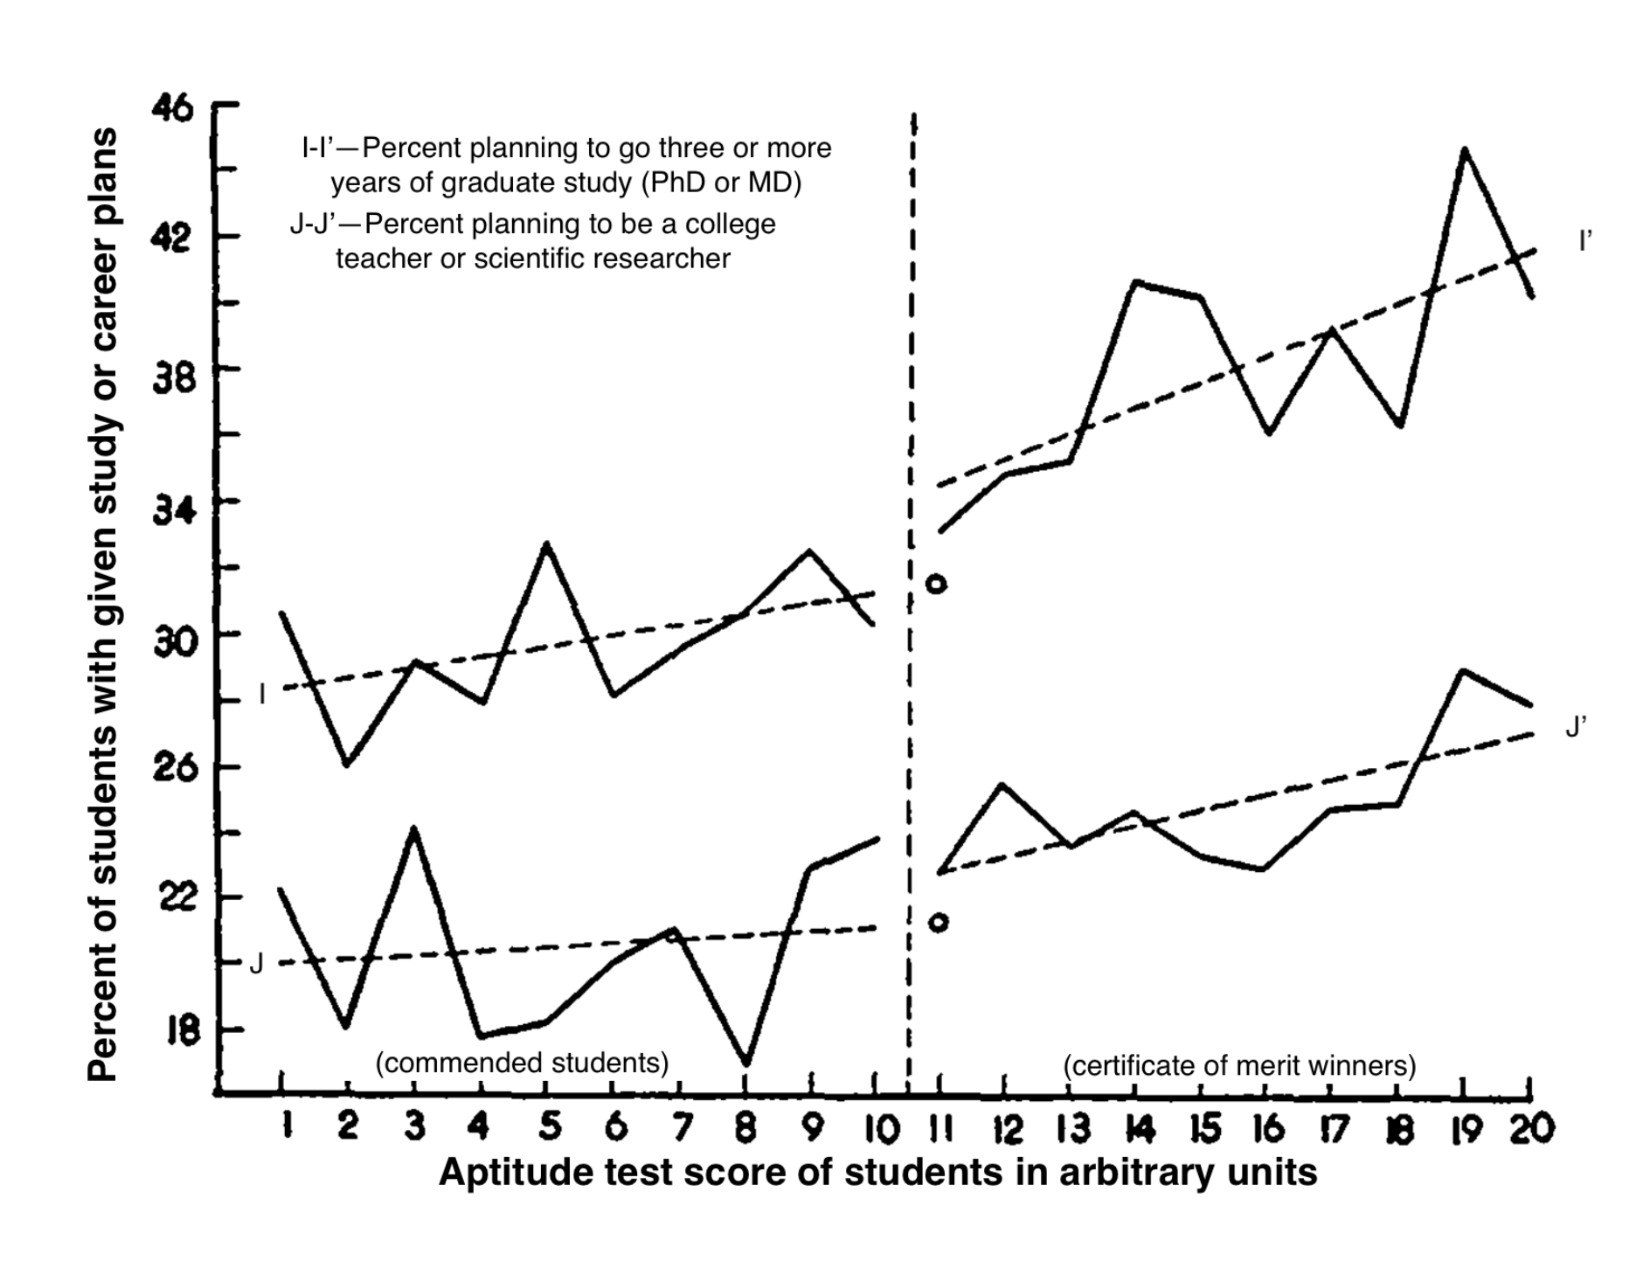
\includegraphics[width = \textwidth]{figures/rdd_graph_1960_modified.pdf}
\caption{改编自 \citet{thistlethwaite1960regression} 的图表，原文中部分文字表述不清，此处略有修改}\label{fig::thistlethwaite1960regression}
\end{figure}

 


\begin{example}
\citet{bor2014regression}使用断点回归研究HIV患者开始抗逆转录病毒治疗的时机对死亡率的影响。是否治疗由患者的CD4计数是否低于200个细胞/$\mu$L决定。CD4细胞是对抗感染的白细胞。
\end{example}




\begin{example}
\citet{carpenter2009effect} 研究了饮酒行为对死亡率的影响，他们以法定最低饮酒年龄作为饮酒行为的“间断点”。该研究所用数据源自美国国家健康统计中心，包含死亡者的出生日期与死亡日期。作者计算了每10万人生存年数中的死亡率，并选用了以下九个变量作为观测指标：
\begin{tabular}{cc}
\hline 
\texttt{all} & 全部死亡案例，即 \texttt{internal} 与 \texttt{external} 之和\\
\texttt{internal} & 因内部原因导致的死亡\\
\texttt{external} & 因外部原因导致的死亡，其余各类死亡因素之和\\
\texttt{homicide} & 他杀 \\
\texttt{suicide} & 自杀\\
\texttt{mva} & 机动车事故致死\\
\texttt{alcohol} & 死亡说明中提及饮酒因素者\\
\texttt{drugs} & 死亡说明中提及药物滥用因素者\\
\texttt{externalother} & 其他外部原因导致的死亡\\
\hline 
\end{tabular}


图 \ref{fig::mlda-9outcomes} 基于 \citet{angrist2014mastering} 所用的数据，呈现了九个指标在21岁阈值处的变化情况。从图中可明显看出，21岁之后死亡率显著上升，这主要源于机动车事故致死率的升高。具体的分析过程留作习题 \ref{hw::MLDA}。 
\end{example}
 

\begin{figure}
\centering
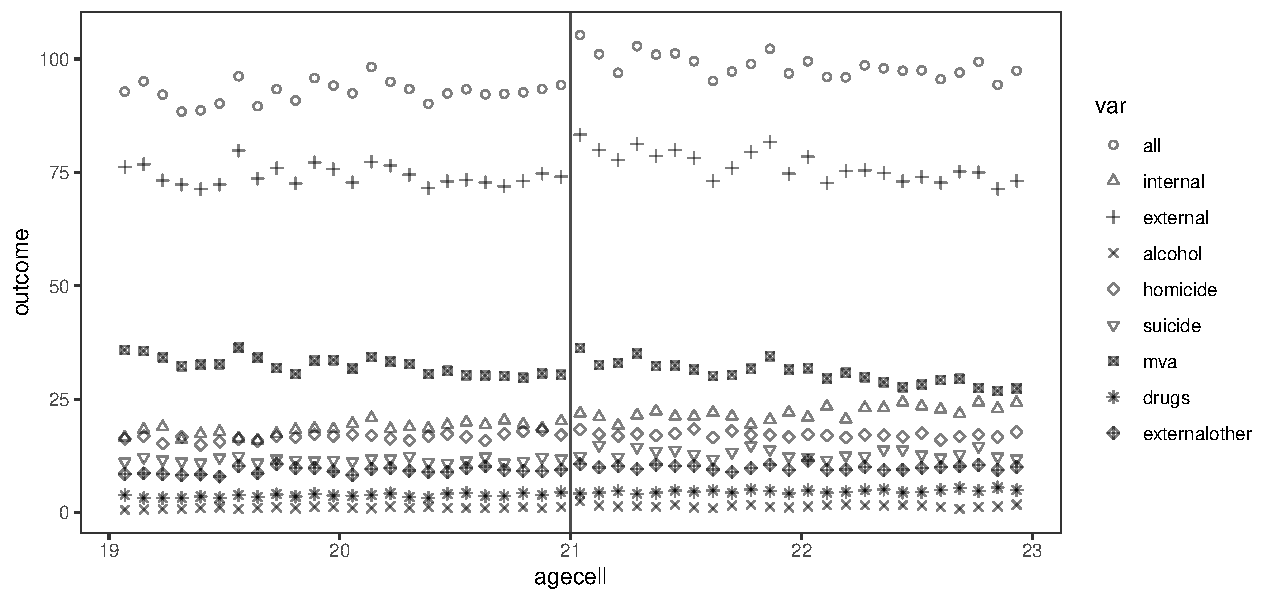
\includegraphics[width = \textwidth]{figures/mlda_9outcomes.pdf}
\caption{基于 \citet{carpenter2009effect} 数据的法定饮酒年龄效应示例}\label{fig::mlda-9outcomes}
\end{figure}


 

 



\subsection{回归间断设计的数学表述}


决定处理的变量$X$，其技术名称是{\it 运行变量}。直观上，断点回归可以识别阈值$x_0$处的{\it 局部平均因果效应}：$$
\tau(x_0) = E\{ Y(1) - Y(0)  \mid X=x_0 \}. 
$$特别地，对于处理下的潜在结果，有\begin{eqnarray}
E\{ Y(1) \mid X=x_0 \} &=& \lim_{\varepsilon \rightarrow 0+ } E\{ Y(1) \mid X=x_0+\varepsilon \} \label{eq::srd-continuity} \\
&=& \lim_{\varepsilon \rightarrow 0+} E\{ Y(1) \mid Z=1, X=x_0+\varepsilon \}  \label{eq::srd-z} \\
&=&  \lim_{\varepsilon \rightarrow 0+} E( Y \mid Z=1, X=x_0+\varepsilon ),
\end{eqnarray}其中若$ E\{ Y(1) \mid X=x\}$在$x_0$处右连续，便得到\eqref{eq::srd-continuity}；\eqref{eq::srd-z}则由$Z$的定义得到。类似地，若$ E\{ Y(0) \mid X=x\}$在$x_0$处左连续，则对照下的潜在结果满足$$
E\{ Y(0) \mid X=x_0 \} =  \lim_{\varepsilon \rightarrow 0+} E( Y \mid Z=0, X=x_0-\varepsilon )
$$因此，可以用这两个极限之差识别$x_0$处的局部平均因果效应。下面总结这一关键识别结果。


\begin{theorem}
\label{thm::identification-rdd}
假设治疗分配规则为 $Z = I(X \geq x_0)$，其中 $x_0$ 为预先设定的阈值。  
再假设 $ E\{ Y(1) \mid X=x\}$ 在 $x_0$ 处右连续，且 $ E\{ Y(0) \mid X=x\}$ 在 $x_0$ 处左连续。此时 $X=x_0$ 处的局部平均处理效应可由下式识别：
$$
\tau(x_0) = \lim_{\varepsilon \rightarrow 0+} E( Y \mid Z=1, X=x_0+\varepsilon ) - \lim_{\varepsilon \rightarrow 0+} E( Y \mid Z=0, X=x_0-\varepsilon ).
$$
\end{theorem}

由于上述公式右侧仅涉及可观测变量，因此参数 $\tau(x_0)$ 可通过非参数方法得以识别。不过该识别公式的形式与我们之前推导出的形式截然不同：这里涉及的是两个条件期望函数的极限值。 



\subsection{阈值附近区域的回归分析}\label{sec::rdd-numerical}

运气较好的话，图形诊断法有时也能清晰呈现阈值处的因果效应。不过多数实际观测数据均存在波动，因此仅凭图形诊断在有限样本下仍显不足。图 \ref{fig::4examples-rdd} 展示了四个模拟示例：前两例在阈值处呈现明显跳跃，后两例则无明显跳跃，不过所有示例的数据生成机制均包含阈值间断特性。 

\begin{figure}
\centering
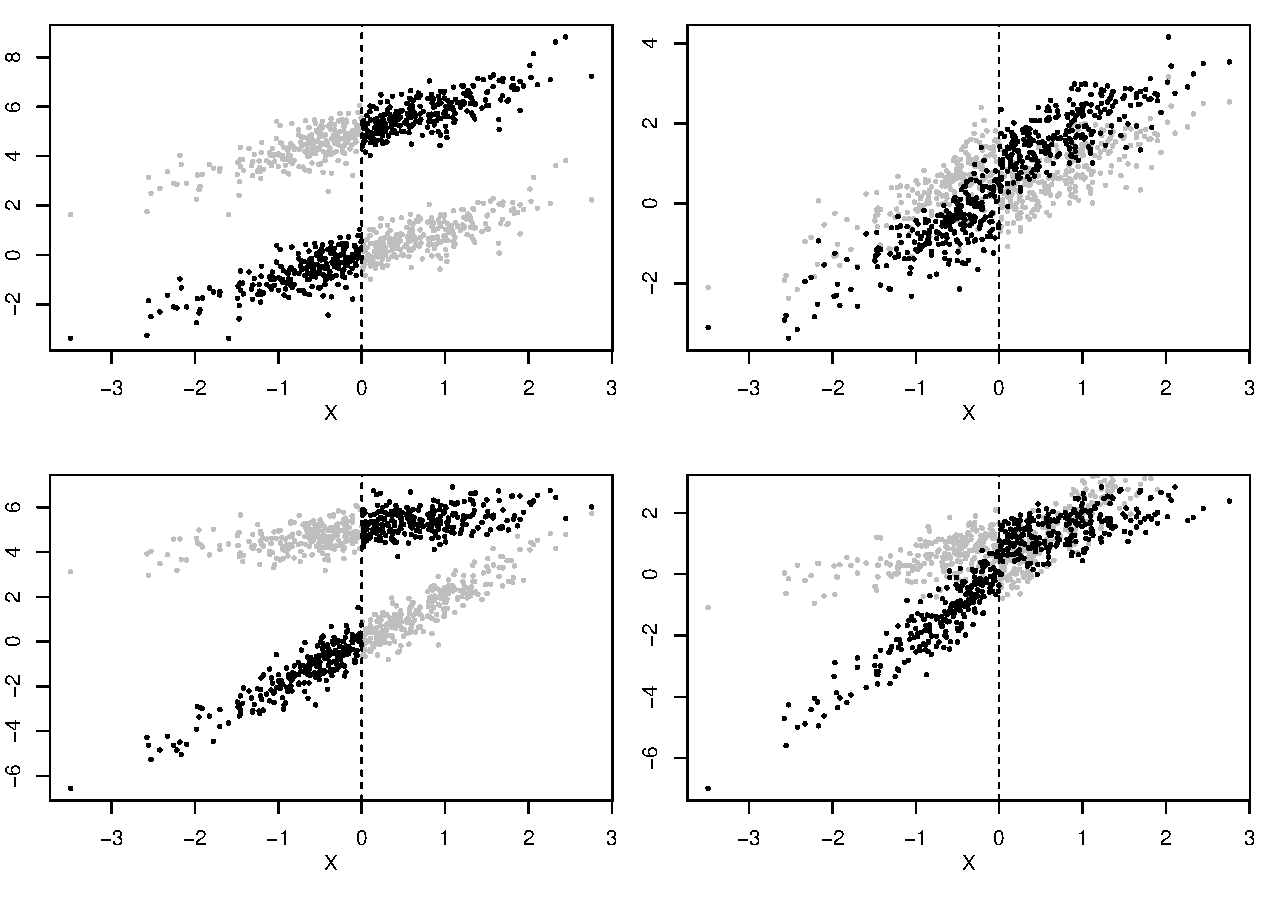
\includegraphics[width = \textwidth]{figures/rdd_graph.pdf}
\caption{断点回归示例。黑点为观测结果，灰点为未观测的反事实结果。第一列的数据生成过程在阈值处产生明显跳跃，第二列的跳跃则不明显。第一行的数据生成过程具有恒定的$\tau(x)$；第二行的$\tau(x)$随$x$变化。}\label{fig::4examples-rdd}
\end{figure}



假设 $E( Y \mid Z=1, X=x ) = \gamma_1 + \beta_1 x$ 与 $E( Y \mid Z=0, X=x ) = \gamma_0 + \beta_0 x $ 是关于 $x$ 的线性函数。此时我们可分别基于治疗组与对照组数据运行最小二乘回归，得到拟合直线 $\hat\gamma_1 + \hat\beta_1 x$ 与 $\hat\gamma_0 + \hat\beta_0 x$。进而可计算 $X = x_0$ 处的平均处理效应估计值：
$$
\hat\tau(x_0) = (\hat\gamma_1 -\hat\gamma_0 ) + (\hat\beta_1 -\hat\beta_0) x_0 .
$$
从数值上而言，$\hat\tau(x_0) $ 与在以下最小二乘回归模型中 $Z_i$ 的系数完全一致：
\begin{eqnarray}
Y_i \sim \{ 1, Z_i, X_i - x_0, Z_i (X_i - x_0)  \} , \label{eq::ols-rdd-1}
\end{eqnarray}
同样的值也对应着下面这个回归模型中 $Z_i$ 的系数：
\begin{eqnarray}
Y_i \sim \{ 1, Z_i,  R_i, L_i \},\label{eq::ols-rdd-2}
\end{eqnarray}
此处 
$$
R_i = \max(X_i - x_0, 0) ,\qquad L_i= \min (X_i - x_0, 0)
$$ 
分别代表了 $X_i - x_0$ 的正负值部分。具体代数推导过程留作习题 \ref{hw::rdd-ols-fits} 讨论。


不过，这种方法可能对违反线性模型假设较为敏感。理论建议只使用阈值附近的局部观测进行回归\footnote{在非参数统计中，这称为{\it 局部线性回归}，属于更广泛的{\it 局部多项式回归}方法\citep{fan2018local}。}。然而，如何选取“局部观测”的规则相当复杂。所幸\ri{R}中\ri{rdrobust}包的\ri{rdrobust}函数实现了多种选择。由于局部观测的选择是断点回归的关键，报告多种选择下的估计值和置信区间似乎更合理。这可视为断点回归的敏感性分析。 


\subsection{实例演示}
\label{section::lee-RDD-example}

\citet{lee2008randomized} 提供了一个著名案例：利用回归间断设计研究美国众议院选举中现任议员的优势所在。  
作者指出：“顾名思义，现任议员即指在上次选举中获胜的政治家。若使其获胜的因素具有相对持续性，那么他们再度当选的可能性理应更高。”由此可见，这确实是一个极具挑战性的因果推断问题。而回归间断设计则堪称研究此类问题的精巧方案。 



运行变量是上一次选举的得票率，并将其中心化到$0$；结果是本次选举的得票率，研究单位为国会选区。处理变量表示某政党是否为该选区当前的执政党，由上次选举的得票情况决定。以下\ri{R}代码生成展示原始数据的图\ref{fig::lee2008}。 

\begin{lstlisting}
house = read.csv("house.csv")[, -1]
plot(y ~ x, data = house, pch = 19, cex = 0.1)
abline(v = 0, col = "grey")
\end{lstlisting}

\begin{figure}
\centering
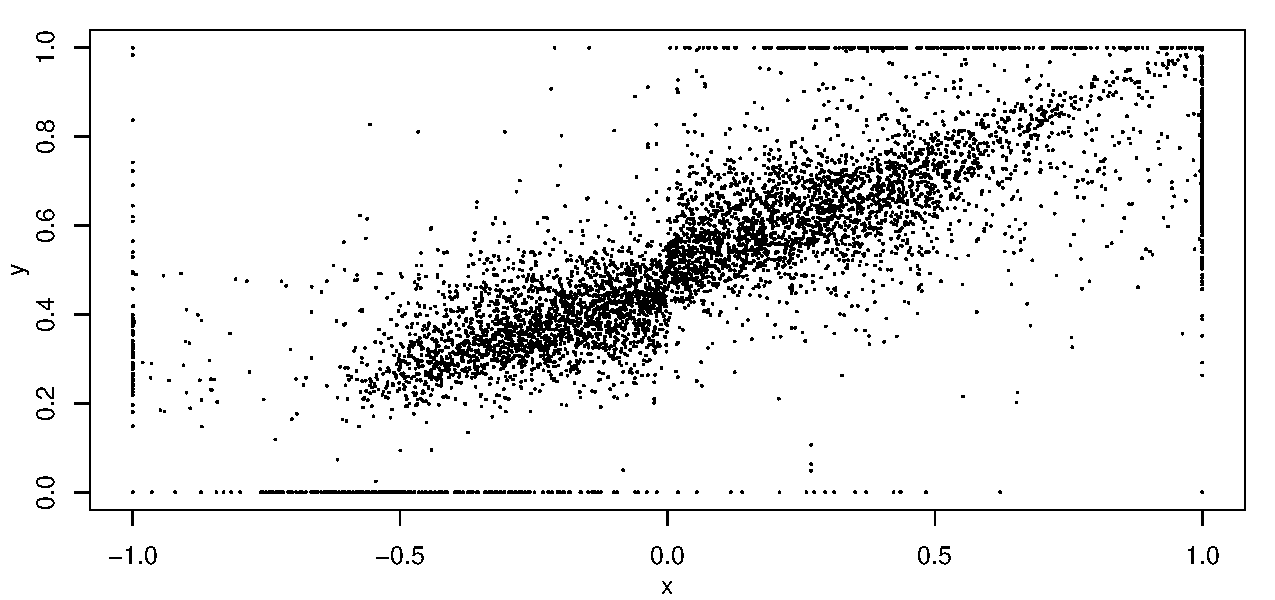
\includegraphics[width = \textwidth]{figures/lee2008rdd.pdf}
\caption{基于 \citet{lee2008randomized} 数据的原始分布图}\label{fig::lee2008}
\end{figure}

 
\ri{rdrobust} 函数可给出三组点估计值与置信区间，均显示现任议员具有显著优势。 

\begin{lstlisting}
> library(rdrobust)
> RDDest = rdrobust(house$y, house$x)
Warning message:
In rdrobust(house$y, house$x) :
  Mass points detected in the running variable.
> cbind(RDDest$coef, RDDest$ci)
                    Coeff   CI Lower   CI Upper
Conventional   0.06372533 0.04224798 0.08520269
Bias-Corrected 0.05937028 0.03789292 0.08084763
Robust         0.05937028 0.03481238 0.08392818
\end{lstlisting}
 
 
 
以下\ri{R}代码还可在按$|X| < h$定义的不同局部观测范围内，通过OLS得到点估计和置信区间。
\begin{lstlisting}
house$z = (house$x >= 0)
hh = seq(0.05, 1, 0.01)
local.lm = sapply(hh, function(h){
  Greg = lm(y ~ z + x + z*x, data = house,
            subset = (abs(x)<=h))
  cbind(coef(Greg)[2], confint(Greg, 'zTRUE'))
})
plot(local.lm[1, ] ~ hh, type = "p",
     pch = 19, cex = 0.3,
     ylim = range(local.lm),
     xlab = "h",
     ylab = "point and interval estimates",
     main = "subset linear regression: |X|<h")
lines(local.lm[2, ] ~ hh, type = "p",
      pch = 19, cex = 0.1) 
lines(local.lm[3, ] ~ hh, type = "p",
      pch = 19, cex = 0.1)
\end{lstlisting}
图 \ref{fig::rdd-lee} 展示了上述估计结果与置信区间随 $h$ 的变化情况。尽管估计值及区间范围对 $h$ 的取值较敏感，但定性结论仍与前述结果一致。 
 
\begin{figure}[h]
\centering
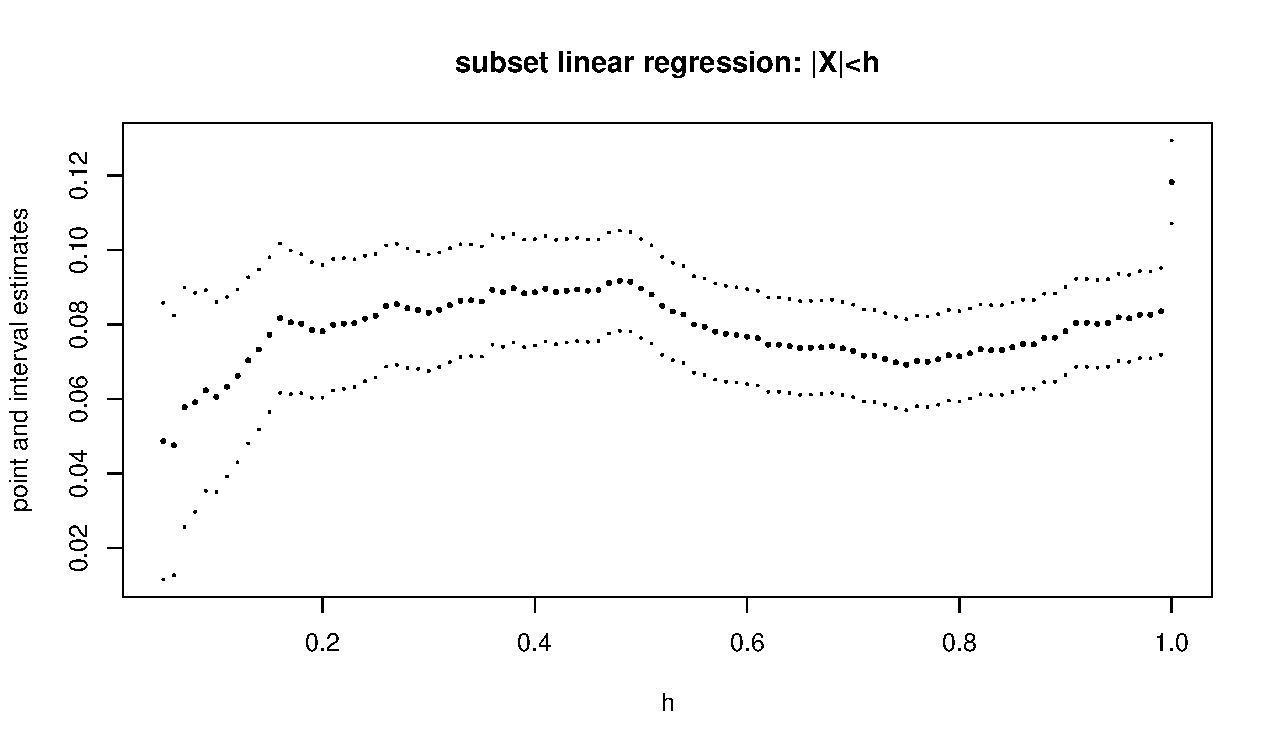
\includegraphics[width = \textwidth]{figures/rdd_lee.pdf}
\caption{基于局部线性回归的估计值与置信区间}\label{fig::rdd-lee}
\end{figure} 
 
 
 
\subsection{回归间断设计的局限性}\label{sec::problems-RD}


回归间断分析可能遇到哪些问题呢？首要的技术难点便是如何精准界定阈值附近的“邻域”。上文已提及此点。

此外，定理 \ref{thm::identification-rdd} 的成立依赖于连续性条件，而现实中该条件可能并不满足。举例来说，若21岁这一阈值处死亡率出现跳跃，则我们未必能将图 \ref{fig::mlda-9outcomes} 中的变化完全归因于法定饮酒年龄调整引发的饮酒行为改变。遗憾的是，这种连续性条件的违背现象很难通过实证方法加以检验。
 
 
\citet{mccrary2008manipulation}提出一种间接检验断点回归有效性的方法，即检查运行变量在阈值处的密度。若其密度在阈值处不连续，可能表明某些单位能够精确操控自身的处理状态。\ri{R}的\ri{rdd}包中，\ri{DCdensity}函数实现了这一检验，细节从略。 


 
 
\section{作业习题}

 

\paragraph{重叠性不足时结果建模的作用定理}\label{hw::outcome-modeling-overlap}

本题是对 \ref{sec::outcome-modeling-overlap} 内容的延伸探讨。我在此陈述一个正式定理。

\begin{theorem}
\label{thm::outcome-overlap}
假设 
$$
Z\ind Y(z) \mid X, \quad (z=0,1)
$$
且
$$
E\{  Y(z) \mid X \} = f_z( r(X)   ),\quad (z=0,1)
$$
其中 $r(X)$ 为某个确定的函数。  
此时平均因果效应 $\tau = E\{ Y(1) - Y(0)  \}$ 可通过以下两式识别：
$$
\tau =E\{   E(Y\mid Z=1, r(X)) - E(Y\mid Z=0, r(X)) \} 
$$
或
$$
\tau = E\left\{   \frac{ZY}{  e(r(X)) }  \right\}  - E\left\{   \frac{(1-Z)Y}{ 1 -  e(r(X)) }  \right\}
$$
此处 $e(r(X)) = \pr\{ Z=1\mid r(X) \}$。 
\end{theorem}

请证明定理 \ref{thm::outcome-overlap}。

说明：当$r(X) = X$时，定理\ref{thm::outcome-overlap}化为平均因果效应的标准IPW公式。当$r(X)$的维度低于$X$时，若$e(X)$的重叠条件不成立、而$e(r(X)) $的重叠条件仍成立，定理\ref{thm::outcome-overlap}就具有更广泛的适用性。 




 \paragraph{线性潜在结果模型}\label{hw::rdd-ols-fits}
 
 
 本题是对 \ref{sec::rdd-numerical} 中数值等价的进一步阐释。 
 
 证明$\hat\tau(x_0) $等于OLS拟合\eqref{eq::ols-rdd-1}和\eqref{eq::ols-rdd-2}中$Z_i$的系数。 
 
% Assume that 
% $$
% Y_i(1) = \gamma_1 + \beta_1 X_i + \varepsilon_i(1),\quad
%  Y_i(0) = \gamma_0 + \beta_0 X_i + \varepsilon_i(0)
% $$
%with $ E\{\varepsilon_i(1) \mid X_i \} =  E\{\varepsilon_i(0) \mid X_i \} = 0$. First, express 
%$$
%\tau(x_0) = E\{ Y_i(1) - Y_i(0)\mid X_i = x_0 \} 
%$$ 
%in terms of the parameters in the above model, and then show that $\tau(x_0)$ can be unbiased estimated by the coefficient of $Z_i$ in the OLS fits of \eqref{eq::ols-rdd-1} or \eqref{eq::ols-rdd-2}.  


提示：先绘制以 $X_i$ 为横轴、$Z_i(X_i - x_0)$、$L_i$ 与 $R_i$ 为纵轴的图像会大有助益。最终结论可通过重新参数化最小二乘回归模型得以验证。 



\paragraph{回归间断设计的模拟分析}

图 \ref{fig::4examples-rdd} 中潜在结果均源自线性模型。现请改用非线性模型进行模拟，并比较不同点估计值与置信区间的表现，尤其关注估计值的偏差、方差以及置信区间的覆盖率等指标。 



\paragraph{法定最低饮酒年龄数据的再分析}\label{hw::MLDA}


图\ref{fig::mlda-9outcomes}展示了阈值处的跳跃。分析\citet{carpenter2009effect}的\ri{mlda.csv}数据。

\paragraph{\citet{lee2008randomized} 数据的鲁棒性再分析}\label{hw::lee2008-robust}

图 \ref{fig::rdd-lee} 呈现了基于同方差假设的置信区间。现请重新绘制图表，使其展示基于 EHW 标准误差的置信区间。 




\paragraph{推荐阅读}

\citet{d2017overlap} 深入探讨了高维协变量条件下重叠性所带来的影响。 

\citet{thistlethwaite1960regression}关于断点回归的原始论文作为\citet{thistlewaiteregression2016obs}再版，并附有许多富有洞见的评论。巧合的是，\citet{thistlethwaite1960regression}和\citet{Rubin:1974}都发表于{\it Journal of Educational Psychology}。
